\documentclass[12pt]{scrartcl}
\usepackage{config}
\usepackage{minted}

%\newcommand\mrh{\color{white}\bfseries}
\newcommand\mrc[1]{\begin{tabular}{@{}l@{}} #1 \end{tabular}}
\setlength\arrayrulewidth{0.8pt}

\usemintedstyle{pastie}

\begin{document}
    \hh{The Splendid Koala}
    
    
    \vspace{10pt}

    
    \hh{Problem}

        You are given a $K \times K$ board, where $K$ is even, and an array $a$ of $N$ pairs of adjacent cells on the board. We say that two cells $\{(r_1, c_1), (r_2, c_2)\}$ are adjacent if $\lvert r_1 - r_2 \lvert + \lvert c_1 - c_2 \lvert = 1$ holds. A set of pairs of adjacent cells is called {\itshape Flamante}\footnote{Flamante means Splendid in spanish :P.} if it is possible to cut the board along the lines that define the cells into two connected, congruent pieces, ensuring that all pairs in the set are strictly within one of the pieces. There is a Koala that loves Flamante sets and would like to know the largest size of a Flamante subset of the $N$ pairs you have. Help our Splendid Koala solve the problem.
        
    \hh{Implementation Details}

       You must implement the function {\itshape Flamante\_Koala()}. This function receives an integer $K$, the size of the board; an integer $N$, the number of pairs of adjacent cells; and four vectors $r1$, $c1$, $r2$, and $c2$, each with $N$ elements, the coordinates of the pairs of adjacent cells. This function must return an integer, the maximum size of a Splendid subset. 
        The function would look like this:

\begin{minted}{c++}
#include <bits/stdc++.h>
using namespace std;

int Flamante_Koala(int K, int N, vector<int> r1, vector<int> c1,
                    vector<int> r2, vector<int> c2) {
    // Implement this function.
}
\end{minted}

    The grader will call the function \textbf{multiple} times for each test case.

    \hh{Examples}
    
        {\itshape Example 1:}
        \begin{itemize}
            \item The grader calls the function 

            \begin{center}
                {\itshape Flamante\_Koala(4, 8, \{1, 2, 3, 4, 1, 2, 2, 4\}, \{2, 2, 2, 2, 4, 1, 2, 1\}, \{1, 2, 3, 4, 2, 3, 3, 4\}, \{3, 3, 3, 3, 4, 1, 2, 2\})}
            \end{center}
            
            \item In this case, returning $7$ would give an accepted verdict. It is possible to show that the set of all pairs is not splendid, but the set with the pairs $\{a_1, a_2, a_3, a_4, a_5, a_6, a_8\}$ is, as shown in the figure:
            \begin{center}
                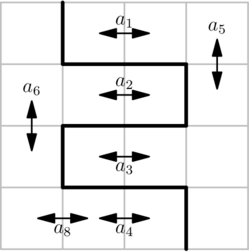
\includegraphics[scale=4]{ej1.png}
            \end{center}
        \end{itemize}
        
        {\itshape Example 2:}
        \begin{itemize}
            \item The grader calls the function 

            \begin{center}
                {\itshape Flamante\_Koala(2, 7, \{1, 2, 1, 1, 1, 1, 1\}, \{1, 1, 1, 1, 2, 1, 2\}, \{1, 2, 1, 2, 2, 2, 2\}, \{2, 2, 2, 1, 2, 1, 2\})}
            \end{center}
            
            \item In this case, returning $4$ would give an accepted verdict. 
        \end{itemize}
        
        {\itshape Example 3:}
        \begin{itemize}
            \item The grader calls the function 

            \begin{center}
                {\itshape Flamante\_Koala(6, 1, \{3\}, \{3\}, \{3\}, \{4\})}
            \end{center}
            
            \item In this case, returning $1$ would give an accepted verdict. 
        \end{itemize}
        
    \hh{Constraints}
        \begin{itemize}
            \item $1 \le N \le 10^5$.
            \item $2 \le K \le 500$. 
            \item $K$ is an even number.
            \item For all $0 \le i \le N - 1$, it holds that $1 \le c1[i], c2[i], r1[i], r2[i] \le K$.
            \item For all $0 \le i \le N - 1$, the cells $(c1[i], r1[i])$ and $(c2[i], r2[i])$ are adjacent.
            \item Let $S_N$ be the sum of the values of $N$ over all calls to the function in a case. It is guaranteed that $S_N \le 10^5$.
            \item Let $S_K$ be the sum of the values of $K$ over all calls to the function in a case. It is guaranteed that $S_K \le 500$.
        \end{itemize}
    
    \hh{Subtasks}


    \begin{itemize}
        \item (10 points) For all $0 \le i \le N - 1$, it holds that $r1[i] = r2[i]$.
        \item (10 points) $N, S_N, K, S_K \le 4$.
        \item (20 points) $N, S_N, K, S_K \le 16$.
        \item (50 points) No additional restrictions.
    \end{itemize}
\end{document}
